\chapter{Funzioni di attivazione}\label{chpt:5}
Le funzioni di attivazione sono molto importanti nelle reti neurali, in quanto introducono la non-linearità nel modello, permettendo di apprendere relazioni complesse nei dati. Senza funzioni di attivazione, una rete neurale profonda risulterebbe equivalente a una semplice trasformazione lineare.

\section{Vanishing Gradient Problem}
Uno dei problemi nell'addestramento delle reti neurali profonde è il \textbf{Vanishing Gradient Problem}, una problematica che viene a verificarsi, quando il gradiente venendo propagato all'indietro diventa molto piccolo, a causa di ciò, smetterà di imparare. È un problema frequente nell'utilizzare funzioni di attivazione come la \textbf{sigmoide} e la \textbf{tangente iperbolica}, poiché visionando i loro grafici, possiamo notare come ci siano grandi tratti dedicati al valore zero e al valore unitario. A causa di questa polarizzazione, i valori non si distinguono fra loro in maniera netta, pertanto tenderanno a scomparire.

\begin{figure}[h]
    \centering
    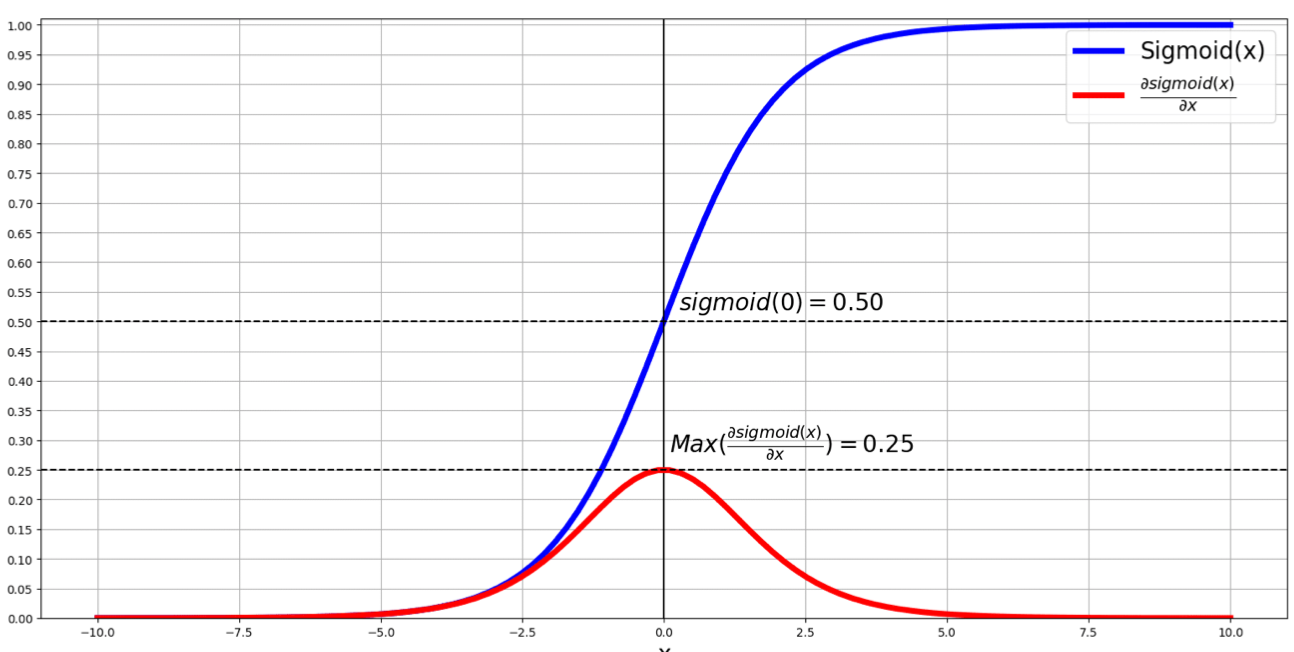
\includegraphics[width=0.85\textwidth]{figure/VanishingGradientProblem.png}
    \caption{Grafico descrittivo del Vanishing Gradient Problem, come possiamo vedere la derivata (in rosso) risulta essere molto ridotta per la gran parte dei valori.}
\end{figure}

\section{Funzioni non saturanti}
Per risolvere il problema, vengono utilizzate funzioni di attivazione dette \textbf{non-saturanti}, come:
\begin{itemize}
    \item \textbf{ReLU (Rectified Linear Unit):} elimina i valori negativi rendendo i calcoli più efficienti, crea però dei problemi legati al gradiente dei valori negativi, rendendoli tutti uguali e anche una mancata derivabilità nell'origine;
    \begin{equation}
        \operatorname{ReLU}(x) = \max(0, x)
    \end{equation}
    \item \textbf{Leaky ReLU:} introduce una piccola pendenza per i valori negativi, riuscendo a ridurre il problema creatosi con la \textit{ReLU};
    \begin{equation}
        \operatorname{LeakyReLU}(x) = \max(\alpha x, x)
    \end{equation}
    \item \textbf{PReLU (Parametric ReLU):} simile a Leaky ReLU, unica differenza è la pendenza dei valori negativi, il quale viene appreso durante l'addestramento, permettendo di avere una pendenza più incisiva;
    \item \textbf{RReLU (Randomized ReLU)}: la pendenza anche qui viene appresa durante l'addestramento, ma si basa su una variabile casuale.
\end{itemize}

\begin{figure}[h]
    \centering
    \begin{tikzpicture}
        \begin{axis}[xlabel={$x$}, ylabel={$f(x)$}, legend pos=north west, domain=-5:5, samples=100, grid]
            \addplot[color=deepblue, thick] {max(0,x)}; \addlegendentry{ReLU}
            \addplot[color=cadmiumorange, thick] {x >= 0 ? x : 0.01*x}; \addlegendentry{Leaky ReLU}
            \addplot[color=deepgreen, thick] {x >= 0 ? x : 0.1*x}; \addlegendentry{PReLU}
        \end{axis}
    \end{tikzpicture}
    \caption{Grafico di ReLU, Leaky ReLU e PReLU, tutti e tre i grafici dopo l'origine si sovrappongono, e seguono lo stesso andamento.}
\end{figure}

\section{Funzioni di Attivazione Avanzate}
Oltre alle funzioni non saturanti, esistono altre funzioni di attivazione avanzate, le quali puntano a gestire diversamente il problema dell'appiattimento dei valori negativi e della non differenziabilità nel punto di coordinata zero:
\begin{itemize}
    \item \textbf{ELU (Exponential Linear Unit):} permette l'utilizzo di valori negativi tramite una decrescita esponenziale, migliorando la stabilità;
    \item \textbf{SELU (Scaled ELU):} nei valori positivi lavora esattamente come una funzione lineare scalata, mentre per quelli negativi si ricurva gradualmente, come succede nella ELU, tuttavia utilizzando un fattore di scala, permettendo di prevenire che i neuroni diventino inattivi;
    \item \textbf{GELU (Gaussian Error Linear Unit):} utilizza una distribuzione gaussiana, utilizzata moltiplicandola per i valori ottenuti e avere delle transizioni più fluide fra i valori positivi e negativi;
    \item \textbf{Softplus}: è un'approssimazione allisciata della funzione rampa vista precedentemente grazie alla funzione non saturante ReLU, la quale permette di avere delle transizioni più dolci.
\end{itemize}

\begin{figure}[h]
    \begin{subfigure}{0.35\textwidth}
        \begin{tikzpicture}[scale=0.65]
            \begin{axis}[xlabel={$x$}, ylabel={$f(x)$}, domain=-5:5, samples=100,grid]
                \addplot[color=deepblue, thick] {x >= 0 ? x : (exp(x)-1)};
                \addplot[color=deepred, thick] {x >= 0 ? x : 1.05*(exp(x)-1)};
            \end{axis}
        \end{tikzpicture}
        \caption{ELU e SELU}
    \end{subfigure}
    \qquad\qquad\quad
    \begin{subfigure}{0.35\textwidth}
        \begin{tikzpicture}[scale=0.65]
            \begin{axis}[xlabel={$x$}, ylabel={$f(x)$}, domain=-5:5, samples=100,grid]
                \addplot[color=deepgreen, thick] {x >= 0 ? x : (exp(x)-1)};
                \addplot[color=cadmiumorange, thick] {0.5*x*(1+tanh(sqrt(2/pi)*(x+0.044715*x^3)))};
            \end{axis}
        \end{tikzpicture}
        \caption{CELU e GELU}
    \end{subfigure}
    \caption{Nel grafico sono rappresentate le varie funzioni di attivazione avanzate, a sinistra, vi è il confronto fra ELU (in blu) e SELU (in rosso), a destra invece il confronto fra CELU (in arancione) e GELU (in verde).}
\end{figure}

Tutte queste funzioni di attivazione, permettono di avere un taglio non netto, fra valori negativi e positivi, garantendo una similarità fra i valori presenti prima e dopo l'origine.

\section{Funzioni Normalizzanti}
Oltre alle moderne funzioni non saturanti, che sono diventate lo standard nella maggior parte delle reti profonde, esiste un'altra categoria di funzioni storicamente importanti o utilizzate in contesti specifici. A differenza delle funzioni come ReLU, il cui scopo principale è introdurre non-linearità mitigando il problema dei gradienti che svaniscono, le funzioni che seguono sono progettate per limitare i valori di output in modi molto specifici. Sebbene alcune di esse, come la funzione soglia (Treshold), siano oggi computazionalmente superate per l'addestramento di reti profonde, la loro comprensione è utile sia dal punto di vista storico sia perché i loro concetti di base riemergono in contesti più avanzati, come la regolarizzazione e l'elaborazione dei segnali.

\begin{itemize}
    \item \textbf{Hardtanh:} la $\operatorname{tanh}$ ha una curva a forma di "S" che si avvicina asintoticamente a $-1$ e $+1$, la $\operatorname{Hardtanh}$ sostituisce questa curva con una funzione lineare a tratti. È una retta con pendenza 1 nell'intervallo $[-1, 1]$ e assume valori costanti al di fuori di questo intervallo. Evita il calcolo di funzioni esponenziali, e sebbene saturi in valori al di fuori dell'intervallo la transizione è netta e non graduale, il che in alcuni contesti può aiutare a gestire meglio il problema dei gradienti che svaniscono;
    \item \textbf{Threshold:} Questa è la funzione di attivazione più semplice e storicamente, la prima ad essere stata utilizzata, fra gli anni '60 e '70, ispirata al modello "tutto o niente" del neurone biologico. Essendo la sua derivata zero, praticamente ovunque, è stata immediatamente rigettata per gli studi sulle rete neurali profonde;
    \item \textbf{Shrink Functions (Tanhshrink, Softshrink, Hardshrink):} Queste funzioni non sono tipicamente usate come attivazioni principali negli strati nascosti, ma piuttosto in contesti di regolarizzazione, sparse coding (codifica sparsa) o elaborazione dei segnali. Il loro scopo è quello di "contrarre" (shrink) i valori di input verso lo zero, eliminando o riducendo il "rumore" di bassa ampiezza.
\end{itemize}

\section{Funzioni Probabilistiche}
Fino ad ora, abbiamo analizzato funzioni di attivazione che operano in modo scalare, ovvero trasformano l'output di ogni singolo neurone indipendentemente dagli altri. Esiste, tuttavia, una classe di funzioni che opera a livello vettoriale, trasformando un intero vettore di output in una distribuzione di probabilità. Queste funzioni sono fondamentali nello strato di output dei modelli di classificazione multiclasse, dove l'obiettivo non è semplicemente ottenere un punteggio per ogni classe, ma interpretare questi punteggi come la probabilità che l'input appartenga a ciascuna di esse. Convertendo i valori grezzi del modello (logits) in probabilità, possiamo non solo selezionare la classe più probabile, ma anche quantificare la fiducia del modello nella sua previsione.

\begin{itemize}
    \item \textbf{Softmax:} questa funzione di attivazione trasforma un vettore in una distribuzione di probabilità all'interno di un range, essa inoltre enfatizza le differenze assegnando a valori più grandi una probabilità più alta, mentre quelli piccoli vengono schiacciati vicino allo zero, la somma di tutti i valori è pari a 1 amplificando la differenza fra i valori scalandoli a elementi dopo la virgola;
    \begin{equation}
        \operatorname{Softmax}(x_i) = \frac{e^{x_i}}{\sum_je^{x_j}}
    \end{equation}
    \item \textbf{Softmin:} la differenza rispetto alla Softmax è l'utilizzo del segno meno all'esponente, dunque una semplice inversione. Questo fa sì che valori più piccoli abbiano una probabilità maggiore, mentre i valori più grandi abbiano probabilità più piccole, essa inoltre è simmetrica rispetto al softmax;
    \begin{equation}
        \operatorname{Softmin}(x_i) = \frac{e^{-x_i}}{\sum_je^{-x_j}}
    \end{equation}
    \item \textbf{LogSoftmax:} quest'altra tipologia di funzione di attivazione invece è una variante della Softmax, in cui si applica il logaritmo alla funzione Softmax per migliorare la stabilità numerica e semplificare il calcolo della perdita nelle reti neurali.
    \begin{equation}
        \operatorname{LogSoftmax}(x_i) =\log( \frac{e^{x_i}}{\sum_je^{x_j}})
    \end{equation}
\end{itemize}

\begin{Osservazione}
    La funzione Softmax può essere vista come la generalizzazione della funzione Sigmoide dal caso binario al caso multiclasse. In altre parole, la Sigmoide è un caso speciale di Softmax quando le classi da predire sono solo due ($K=2$).
\end{Osservazione}
